\renewcommand{\algorithmicrequire}{\textbf{Input:}}
\renewcommand{\algorithmicensure}{\textbf{Output:}}

\section{System Framework}\label{sec:SDI}
We illustrate how EarnCache works in this section. Firstly we present the overview about the caching mechanism of EarnCache, and then discuss its architecture design, and finally explain the incremental cache-earning policy and its implementation.

\subsection{Overview}\label{sec:overview}

On shared non-big clusters with relatively limited cache capacity, cache resource conflicts would be normal.
When only few users are using a non-big cluster and the competition for cache resources is mild, applying on-demand caching could expedite hotter blocks taking over cache resources from colder blocks, and hotter data is less likely to be cached out by colder data. When more concurrent users consume the cluster and competition for cache resources gets wild, on-demand caching leaves concurrent cache resource demands unmediated, making hotter data more vulnerable to being cached out. 
Files which are frequently accessed recently sometimes could be totally cached out by files which would rarely be accessed for the second time in near future, then these hot cached-out files require to be cached in soon as their next access should occur in the upcoming future. We consequently need to revisit existing on-demand caching mechanisms and strategies, and propose more effective measures to improve the efficiency of data caching on non-big clusters.

We believe that a good caching strategy for non-big clusters should be self-adaptive to resource competition conditions, depressing competitions and preventing thrashings when resources are in desperate deficit.
Obviously caching big data files on demand as a whole could not provide such self-adaptivity. 
Not compulsorily caching files entirely provides the elasticity of tuning the amount of cache resources allocated for different files based on their access recency and frequency.

Ideally, more recently frequently accessed files should be assigned with more cache resources, and less recently frequently accessed ones should be assigned with less cache resources. 
However, it's not possible to know in advance what files would be frequently accessed in the upcoming future,
and we could only make predictions based on historical file access patterns, especially the most recent information. Based on files' historical access information, EarnCache implements an incremental caching strategy, where a user should earn resources to cache files from other concurrent users via accessing these files. Cache resources are incrementally allocated to files that become more frequently accessed, which gradually takes over cache resources, until all blocks of the file have been cached in. The more a file is accessed, the more cache resources it takes over. 
The incremental caching strategy ensures that files occupying cache resources are recently frequently accessed and will not be flushed out by files that are only accessed occasionally or randomly.


\subsection{Architecture}\label{sec:Arch}
Files originally reside in under distributed file system (e.g. Hadoop File System), and EarnCache coordinately caches them across the whole cluster. EarnCache consists of a central \emph{master} and a set of \emph{workers} residing on storage nodes as shown in Figure.~\ref{fig:Arch}. The \emph{master} is responsible for: ~1) determining how many cache resources should be allocated to a file based on recent file access information; ~2) informing workers of the cache resource allocation plans via heartbeats; ~3) keeping track of metadata of which storage node a cached block resides on; ~4) answering clients' queries on cache metadata. 
And a \emph{worker} is responsible for: ~1) receiving the resource allocation plan from master; ~2) calculating how many resources a file should contribute to compose the allocated resources; ~3) caching in/out blocks according to the calculated resource composition plans; ~4) informing the master of cached blocks via heartbeats; ~5) serving clients with cached blocks.

As illustrated in Figure.\ref{fig:Arch}, a client accesses a block in the following procedures: ~1) the client queries the master where the block is located; ~2) the master tells the client which worker the requesting data resides on; ~3) the client contacts the worker to access the block; ~4) the worker serves the client with the block data from cache. 
One thing worth noting here is that: the client will not contact any worker to access a block if the block is not in cache of any worker nodes, as the master only keeps track of cached blocks.
In this situation, the client has to fetch data from the under file system.


\begin{figure}[!htbp]
\centering
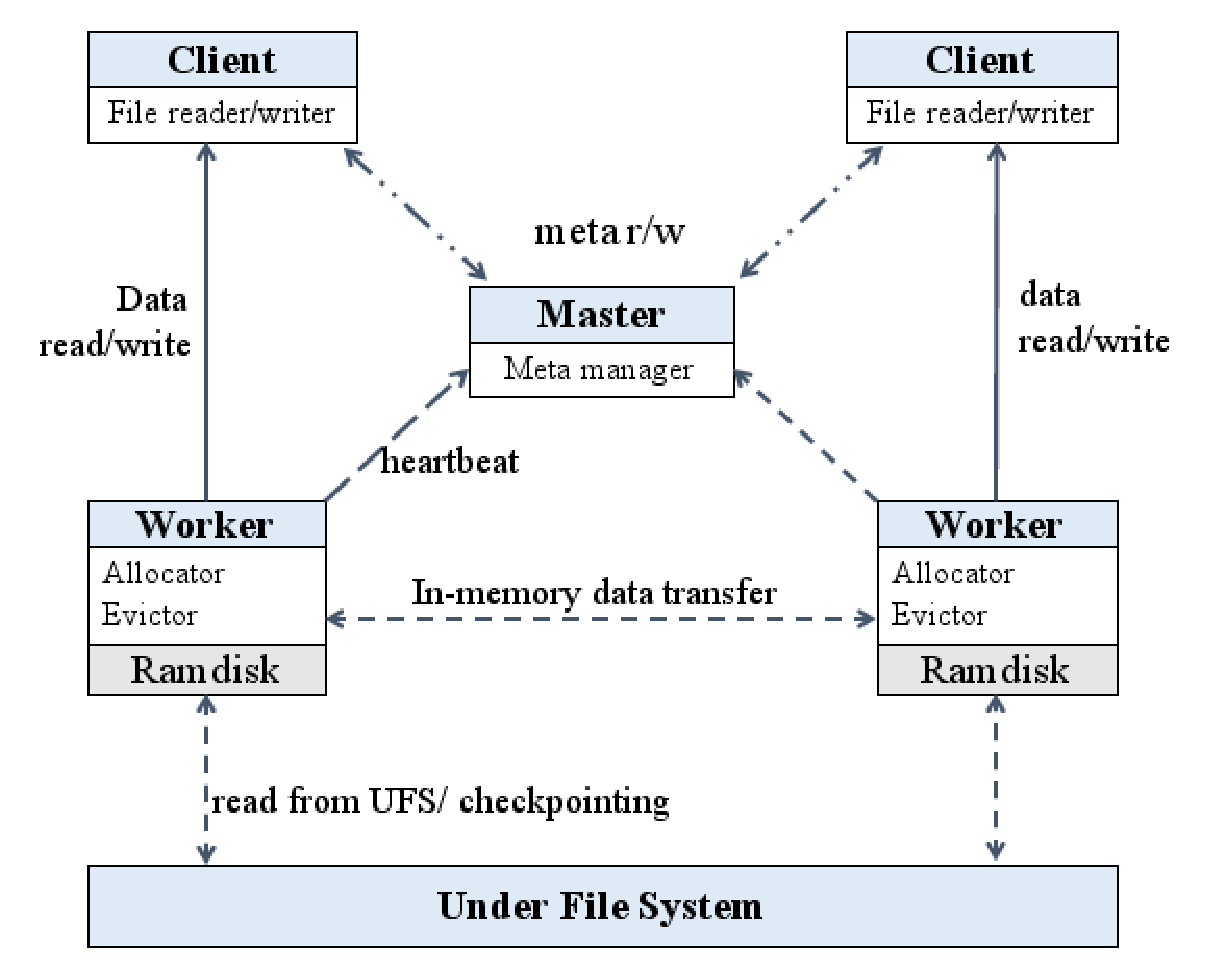
\includegraphics[scale=0.40]{figures/architecture.eps}
\caption{EarnCache's Architecture.}
\label{fig:Arch}
\end{figure}

%Competition for computational resources rarely influences the completion of running tasks, namely each of the scheduled concurrent tasks may run as fast as it runs alone. does not have obviously decrease computation efficiency, as ; while competition for cache resources may seriously decrease cache efficiency, because of data caching in/out cost.
%Big data applications usually access files in a scan fashion and datasets are usually prohibitively huge in size.
%Work about on-demand caching mainly focuses on cache replacement policies, and most replacement policies are variants of LRU, LFU or LRU-LFU-combined.

\subsection{Incremental Caching}\label{sec:framework master}

As we prefer recently frequently accessed files incrementally taking over resources from less recently frequently accessed files, "recently" should be defined quantitatively before we could design the incremental caching strategy, and other related elements should also be clarified. Table.~\ref{tab:notation} presents all definitions of notations involved in our incremental caching strategy.
\begin{table}[!htb]
	\caption{Notation definitions}
	\label{tab:notation}
	\centering
	\begin{tabular}{|p{0.15\linewidth}|p{0.75\linewidth}|}
		\hline
		Notation & Definition\\
		\hline
		$W$ & predefined window size of the most recently accessed data for observing files falling within\\
		\hline
		$a,b$ & scan time per unit data from memory(a) and hdd(b) \\
		\hline
		$N$ & total number of files falling in the observation window\\
		\hline
		$d_i$ & data size of the $i$th file\\
		\hline
		$D$ & total data size of $N$ files\\
		\hline
		$M$ & cache capacity of the whole cluster\\
		\hline
		$f_i$ & access frequency of the $i$th file\\
		\hline
		$F$ & total access frequency of $N$ files\\
		\hline
		$x_i$ & percentage of data cached for the $i$th file\\
		\hline
		$h_i(x_i)$ & the $i$th file's profit gain with $x_i$ data cached\\
		\hline
	\end{tabular}
\end{table}

We define a function $h_i(x_i)$ to denote the profit gain of the $i$th file to instruct how cached files should contribute resources. Then we attempt to instantiate $h_i(x_i)$ and to maximize total profit gain of all files falling in the observation window, just as Equ.\ref{optimization target} shows.
\begin{equation}\label{optimization target}
\sum_{i=1}^{N} f_i \cdot h_i(x_i) \
\end{equation}

According to definitions in Tab.\ref{tab:notation}, we can assume that the time it takes to scan the $i$th file is:
\begin{equation}\label{time}
time(x_i)=[a\cdot x_i+b\cdot (1-x_i)]\cdot d_i
\end{equation}

As mentioned above, we use $h_i$ to indicate the $i$th file's profit gain with $x_i$ data cached. If we take saved scan time as a file's profit gain, then we can define $h_i$'s deviation at $x_i$ as its gain change over $\delta x_i$, which could be further defined as the percentage of increased saving of the file's scan time with increased cache share at $x_i$ over the total saved scan time at $x_i$, compared to zero cache share, just formulized as:
\begin{equation}\label{dhi}
\frac{\delta h_i}{\delta x_i}=\frac{time(x_i) - time(x_i+\delta x_i)}{time(0) - time(x_i)}=\frac{\delta x_i}{x_i}
\end{equation}

Thus we can derive that $h_i(x_i)=\ln x_i$, and now our optimization goal becomes
\begin{equation}
\sum_{i=1}^{N} f_i \cdot \ln x_i
\end{equation}
subjected to
\begin{equation}
\sum_{i=1}^{N} x_i\cdot d_i \leq M
\end{equation}

Note that at any given time,  $x_i$ is the only variant contained in the optimization goal, and $f_i \cdot \ln x_i$ is a convex function. After applying Lagrange multiplier method, our maximizing goal turns to:
\begin{equation}
L=\sum_{i=1}^{N} f_i\cdot \ln x_i - \lambda (\sum_{i=1}^{N} x_i\cdot d_i - M)
\end{equation}
Let $\frac{\delta L}{\delta x_i}$ be 0, then we get
\begin{equation}\label{xi result}
x_i\cdot d_i= \frac{f_i}{F} \cdot M
\end{equation}

The above result shows that the amount of memory resources allocated to a file is linear to $f_i$ at a given moment, as all files' access frequency is determined at that moment, which exactly responds to our original intention of incremental caching. 
One more thing worth noting is that: if the overall size of files filling in the whole observation window is smaller than the cache capacity, i.e. there are cache resources being occupied by files that are not in the observation window, EarnCache will collect resources from those obsolete files by LRU when there is a caching request,
and the requesting file could cache in its blocks once and for all, rather than gradually taking over resources from files falling within the observation window. 
EarnCache thereby could adaptively devolve to traditional on-demand-caching so as to expedite the process of collecting cache resources for actively accessed files 
when contention for cache resources is light, and evolve to incremental caching to depress competition when resources are in deficit.

\subsection{Implementation Details}\label{sec:share and fair}

We implemented EarnCache by implanting our incremental caching mechanism into the modified Tachyon\cite{tachyon}. In EarnCache, we first evenly re-distribute a file's cached data blocks across the whole cluster, so that almost the same amount of blocks are hosted in cache on each cluster node, and all workers can manage their cache resources independently yet still in concert. As uneven data distribution will drag down completion of the whole job, evenly distributing cached data blocks guarantee that tasks running on each node could ideally finish almost simultaneously.

When the $i$th file needs caching, EarnCache pre-allocates ${f_i}/{F}$ fraction of cache resources on each node to the file based on Equ.\ref{xi result}. If resources pre-allocated to the file is more than its aggregated demands, EarnCache has other files in need of cache resources fairly share the spare cache. 
Each worker checks its available cache resources, and allocates as many as possible to them directly, which could make full use of cache resources. 
When there are not enough resources available, the worker calls \emph{BlocksToEvict()}, which implements the eviction algorithm with incremental caching, to determine which blocks should be cached out. 
%As all blocks are cached in from the underlying file system, cached-out blocks need no more backup and workers could discard them directly from cache. After blocks being cached in/out, 
When evicting process is done, the worker will inform the master to update the metadata.

Alg.~\ref{worker algorithm} describes the process of evicting blocks. EarnCache first checks whether the file requesting cache resources has used up its pre-allocated share in Line 1$\sim$3. In the while loop, Line 7$\sim$14 mainly selects files who has overcommitted the most cache resource. If no such file exists, EarnCache will reject the cache request (Line 15$\sim$17). Otherwise, blocks of these selected files are added to the candidate block set until enough cache resources have been collected(Line 18$\sim$24). 
As recency and frequency of all blocks within a file are identical, 
workers do not differentiate between blocks of the same file when selecting blocks to cache out.
Note that by snatching cache resources from most over-consumed files, EarnCache ensures that increased cache occupation of file $r$ causes least degradation of other files' cache occupation amount.

%By snatching cache resource from most over-consumed files, EarnCache ensures that increased cache occupation of file $r$ causes less degradation of other files' cache amount considering the pre-allocation plan.

\begin{algorithm}[!htb]
	\caption{Eviction Algorithm: BlocksToEvict()}
	\label{worker algorithm}
	\begin{algorithmic}[1]
		\Require \emph{s}, requested cache resources; \emph{r}, the requesting file id; \emph{A=\{$a_1$, $a_2$...$a_N$\}}, a list of files' pre-allocated memory bytes; \emph{C=\{$c_1$, $c_2$...$c_N$\}}, a list of current consumed memory bytes in local node; \emph{M}, memory capacity of local node
		\Ensure a list of candidate blocks to evict
			
		\If {$c_r \ge a_r$}
			\State algorithm ends as file r has already consumed all its allocated memory
		\EndIf
		\State $candidate \gets \{\}$ \Comment \textit{candidate cached out blocks}
		\State $mem \gets 0$ \Comment \textit{free resources obtained from evicting candidates}
		\While {$mem < s$}
		\State $j \gets -1$
		\State $over_j \gets 0$
		\For {$a_i$ in $A$ and $i \ne r$}
			\If {$c_i - a_i > over_j$}
				\State $j \gets i$
				\State $over_j \gets c_i - a_i$
			\EndIf
		\EndFor
		\If {$j = -1$}
			\State return as request failure
		\EndIf
		\State find $b_j$ as a block of file $j$ and not in $candidate$
		\State $candidate \gets candidate + b_j$
		\State $mem \gets mem + size of (b_j)$
		\State $c_j \gets c_j - sizeof(b_j)$
		\If {$mem \ge s$}
			\State return $candidate$
		\EndIf
		\EndWhile
		
	\end{algorithmic}
\end{algorithm}

%\begin{figure}[!htb]
%	\centering
%	\label{fig:decision-making}
%	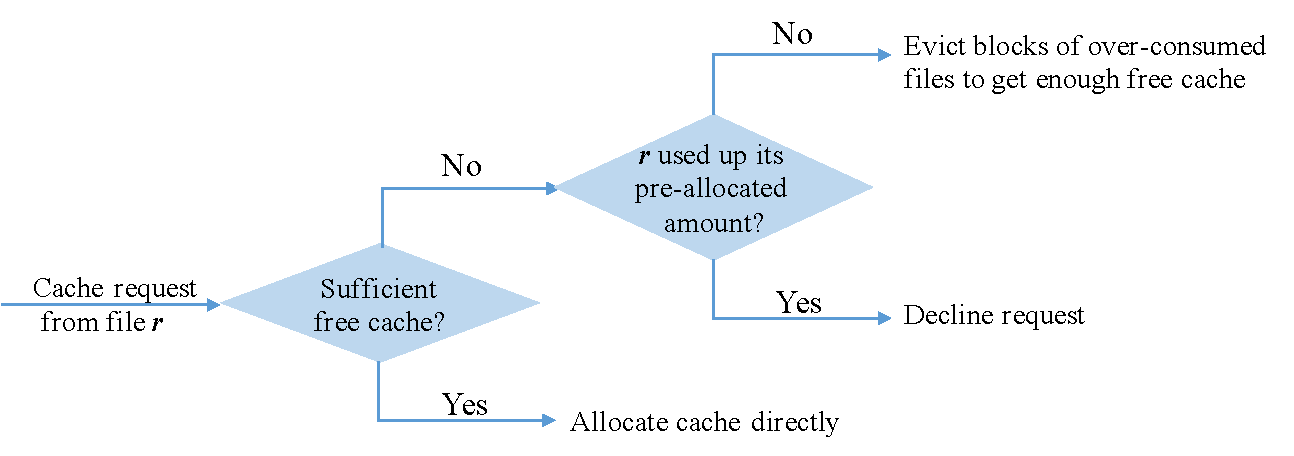
\includegraphics[scale=0.70]{figures-final/decision-making.pdf}
%	\caption{The decision-making process of EarnCache when a new cache space request occurs.}
%\end{figure}


